We wish to solve equations by using analogue components, and the heart of many of these systems is an operational amplifier which amplifies the signals inputted into it, but it is highly used in analogue components due to its versitility. It has three key properties which are seen to be observed and are essential to its operation. They are:

\begin{itemize}
  \item Very High Gain ($V_{in} = V_{out}/Gain = 0$)
  \item Very High Input Impedance ($I_{in} = V_{in}/ R_{in}$)
  \item Very Low Output Impedance ($V_{out}$
\end{itemize}

%% Here I figure we should derive the circuit and then write up generally how it works for each circuit.

\subsection{Summing}

\begin{figure}[ht!]
\centering
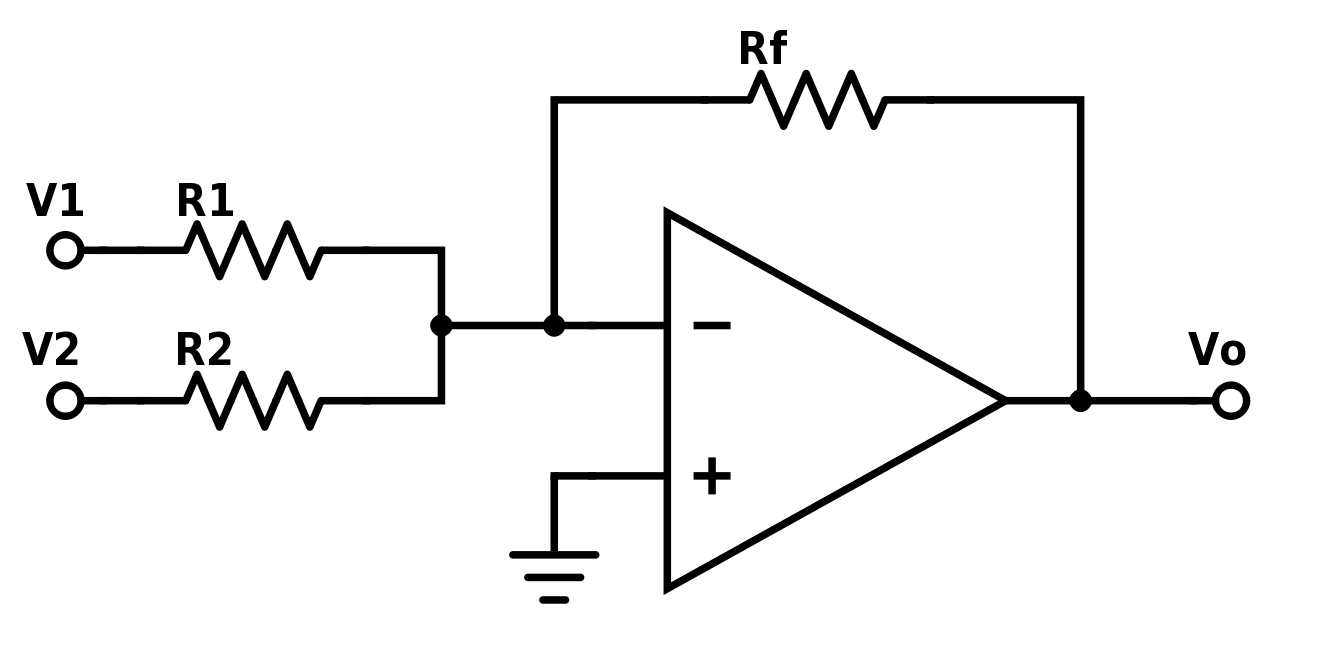
\includegraphics[scale=.15]{figures/460-17-1-Summer.png}
\caption{The circuit diagram used for summing signals from two inputs together}
\label{fig:CD_Sum}
\end{figure}


\subsection{Differentiation}

\begin{figure}[ht!]
\centering
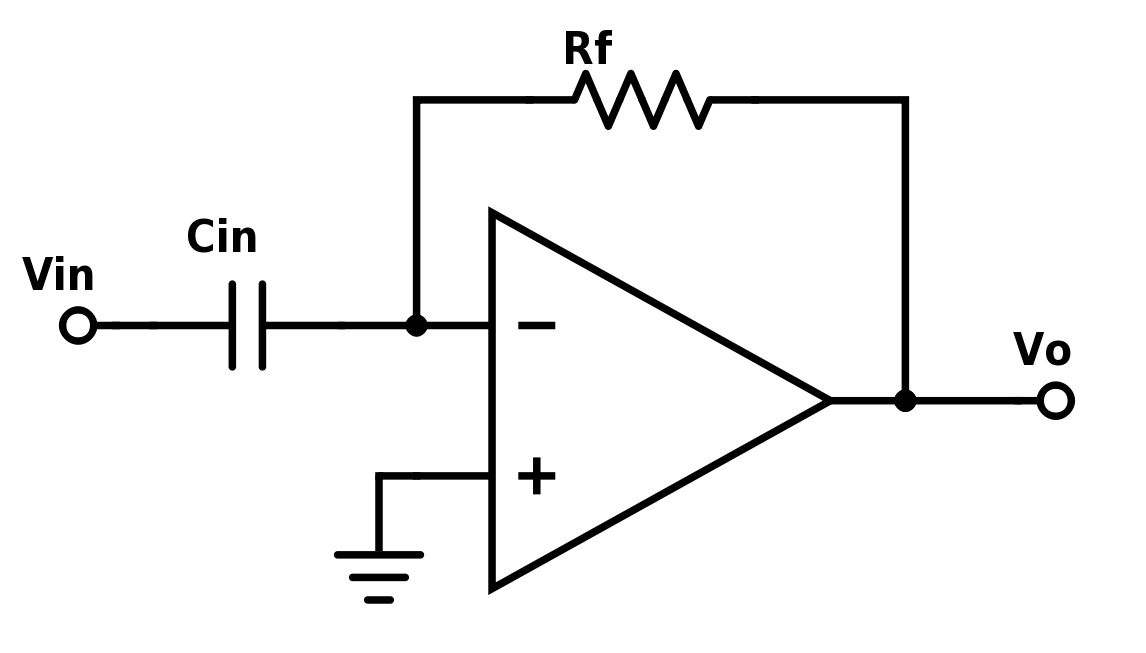
\includegraphics[scale=.25]{figures/460-17-2-Differentiator.png}
\caption{The circuit diagram used for Differentiating a signal}
\label{fig:CD_Diff}
\end{figure}

\subsection{Integration}

\begin{figure}[ht!]
\centering
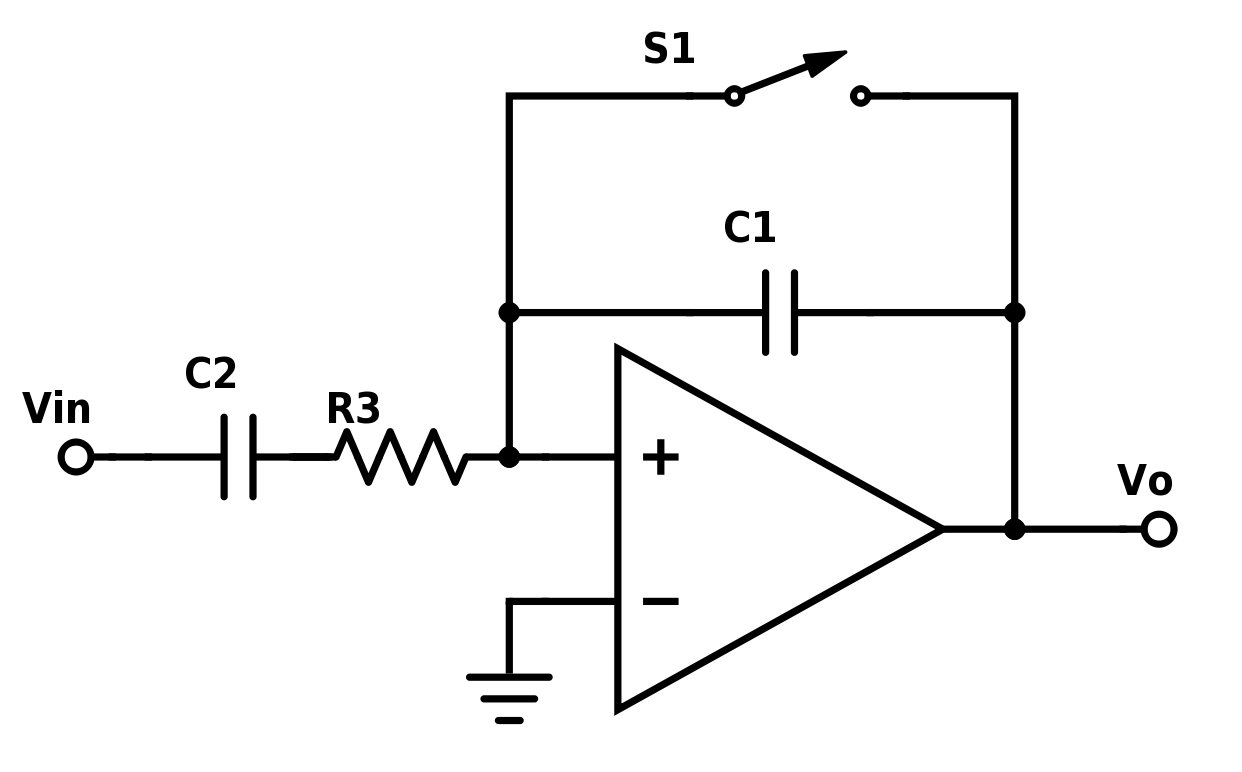
\includegraphics[scale=.20]{figures/460-17-3-Intergrator.png}
\caption{The circuit diagram used for integrating a signal}
\label{fig:CD_Int}
\end{figure}

\subsection{Exponential}

\begin{figure}[ht!]
\centering
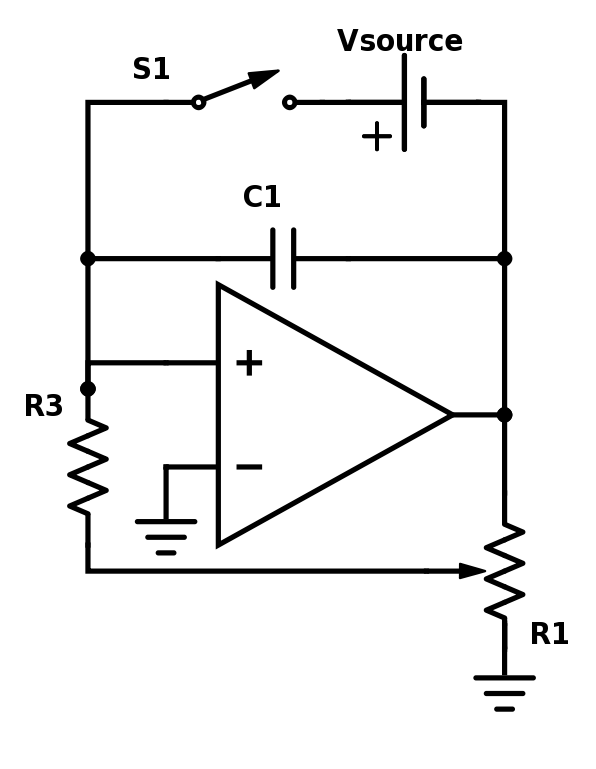
\includegraphics[scale=.33]{figures/460-17-4-Exponential.png}
\caption{The circuit diagram used for creating the solution to the exponential equation}
\label{fig:CD_Exp}
\end{figure}

\subsection{Damped Harmonic Motion}

\begin{figure}[ht!]
\centering
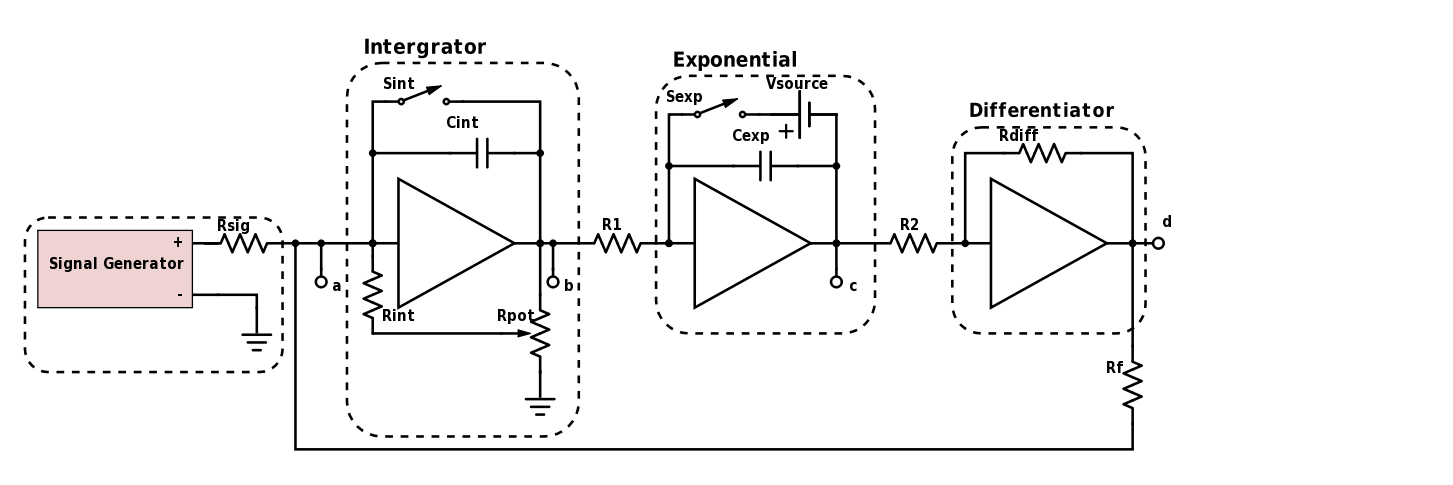
\includegraphics[scale=.4]{figures/460-17-6-Forced-HO.png}
\caption{The circuit diagram which is used for making the solution to the Damped Harmonic Oscillator}
\label{fig:CD_HO}
\end{figure}

\subsection{Forced Damped Harmonic Motion}